%!TEX root = ../terrainbook.tex

\graphicspath{{spatialextent/}}

\chapter{The spatial extent of a point cloud}
\label{chap:spatialextent}

\begin{figure}[h]
  \centering
  \begin{subfigure}[b]{0.21\linewidth}
    \centering
    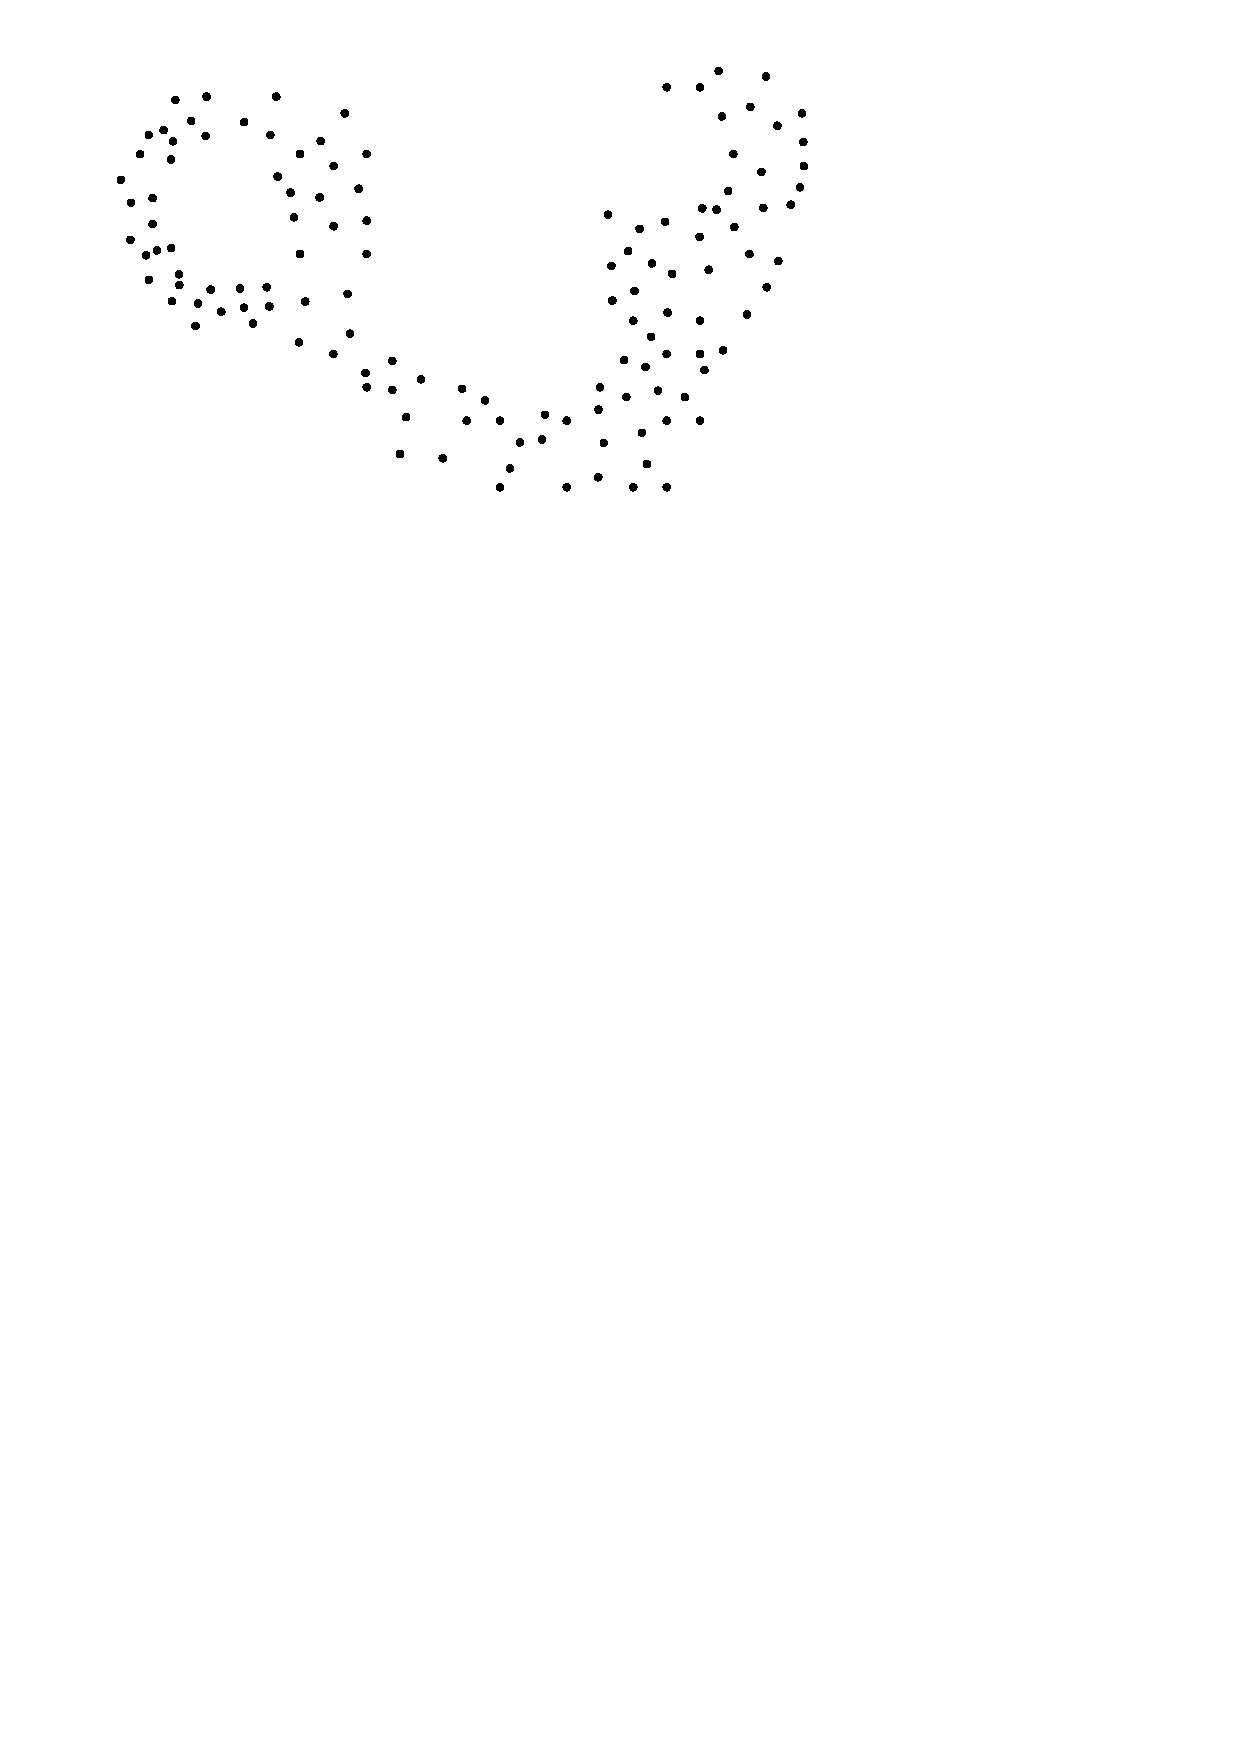
\includegraphics[page=1,width=\textwidth]{figs/idea.pdf}
    \caption{A set of points in $\mathbb{R}^2$}
  \end{subfigure}%
  \qquad
  \begin{subfigure}[b]{0.21\linewidth}
    \centering
    \includegraphics[page=2,width=\textwidth]{figs/idea.pdf}
    \caption{Its convex hull}
  \end{subfigure}
  \qquad
  \begin{subfigure}[b]{0.21\linewidth}
    \centering
    \includegraphics[page=3,width=\textwidth]{figs/idea.pdf}
    \caption{A $\chi$-shape}
  \end{subfigure}%
  \qquad
  \begin{subfigure}[b]{0.21\linewidth}
    \centering
    \includegraphics[page=4,width=\textwidth]{figs/idea.pdf}
    \caption{An $\alpha$-shape}
  \end{subfigure}
\caption{Different methods to obtain the spatial extent of a given set of points in the plane.}
\label{fig:ideas}  
\end{figure}

Given a point cloud, one operation that practitioners need to perform is to define the spatial extent of the dataset.
That is, they need to define the shape of the region that best abstracts the set of points; in the context of terrains this region is often in two dimensions.
% , which is represented by a one or more polygons,
This is useful for instance to calculate the area covered by a dataset, to convert it to other formats (\eg\ raster), to get a quick overview of several datasets it is faster to load a few polygons and not billions of points, etc.

%

The spatial extent is often called: envelope, hull, concave hull, or footprints.
It is important to notice that the spatial extent is not uniquely defined and can a vague concept, as Figure~\ref{fig:ideas} shows there are several potential regions for a rather simple set of points, and most of these could be considered `correct' by a human.

%

We present in this chapter a few methods/algorithms that are used in practice to define the spatial extent of a set of points in $\mathbb{R}^2$, which implies that the points in a point cloud are projected to the plane.

% TODO : linear approximation only here


%%%%%%%%%%%%%%%%%%%%
%
\section{Properties of the region}
\label{sec:properties}

Let $S$ be a set of points in $\mathbb{R}^2$, and $R(S)$ the region that characterise the spatial extent of $S$.
The region is potentially formed by a set of polygons (if $S$ forms two distinct clusters for instance) and in practice most algorithms will computer a linear approximation of $R(S)$, so the polygons will have straight edges as boundaries.

To evaluate the different algorithms, we list here different properties that one must consider when defining the spatial extent of a set of points.
\begin{description}
  \item[P1.] \textbf{Polygons need to be \emph{regular}?} Are polygons allowed to have dangling parts (lines), such as the one in Figure~\ref{fig:properties}b
  \item[P2.] \textbf{Are points allowed to be on the boundary of the region?} All of the regions in Figure~\ref{fig:properties} (except d) have points on the boundary of $R(S)$.
  \item[P3.] \textbf{All points part of the region?} Can outliers be ignored? Or do they have to be part of the region? In Figure~\ref{fig:properties}a they are all part, in Figure~\ref{fig:properties}b--e one outlier is not (if we consider that $S$ represents the letter ``b'').
  \item[P4.] \textbf{Region is one connected component?} Or are more components allowed? In Figure~\ref{fig:properties}a--d there is one component, but Figure~\ref{fig:properties}e has two.
  \item[P5.] \textbf{Are holes allowed in a polygon?} Polygons in Figure~\ref{fig:properties}a/c/d have only an exterior boundary, while in Figure~\ref{fig:properties}e one polygon has an interior boundary too (a hole).
  % TODO : do we speak of time complexity of each algorithm? 
\end{description}
\begin{figure}
  \centering
  \begin{subfigure}[b]{0.15\linewidth}
    \centering
    \includegraphics[page=2,width=\textwidth]{figs/properties.pdf}
    \caption{}
  \end{subfigure}%
  \qquad
  \begin{subfigure}[b]{0.15\linewidth}
    \centering
    \includegraphics[page=4,width=\textwidth]{figs/properties.pdf}
    \caption{}
  \end{subfigure}
  \qquad
  \begin{subfigure}[b]{0.15\linewidth}
    \centering
    \includegraphics[page=5,width=\textwidth]{figs/properties.pdf}
    \caption{}
  \end{subfigure}%
  \qquad
  \begin{subfigure}[b]{0.15\linewidth}
    \centering
    \includegraphics[page=6,width=\textwidth]{figs/properties.pdf}
    \caption{}
  \end{subfigure}
  \qquad
  \begin{subfigure}[b]{0.15\linewidth}
    \centering
    \includegraphics[page=3,width=\textwidth]{figs/properties.pdf}
    \caption{}
  \end{subfigure}
\caption{Different properties for the spatial extent}
\label{fig:properties}  
\end{figure}


%%%%%%%%%%%%%%%%%%%%
%
\section{Convex hull}

As explained in Section~\ref{sec:convexhull}, given $S$ a set of points in $\mathbb{R}^2$, its convex hull, denoted here conv($S$), is the minimal convex set containing $S$.
Two examples of convex hulls are in Figures~\ref{fig:ideas}b and~\ref{sec:properties}a.

%

For a given set of points, the convex hull is uniquely defined and does not require any parameters (unlike the other methods listed below).
It is also relatively easy to compute: it can be extracted from the Delaunay triangulation, or there exists specific algorithms.
One of them is the well-known \emph{gift wrapping algorithm}, shown in Figure~\ref{fig:giftwrapping}.
\begin{figure}
  \centering
  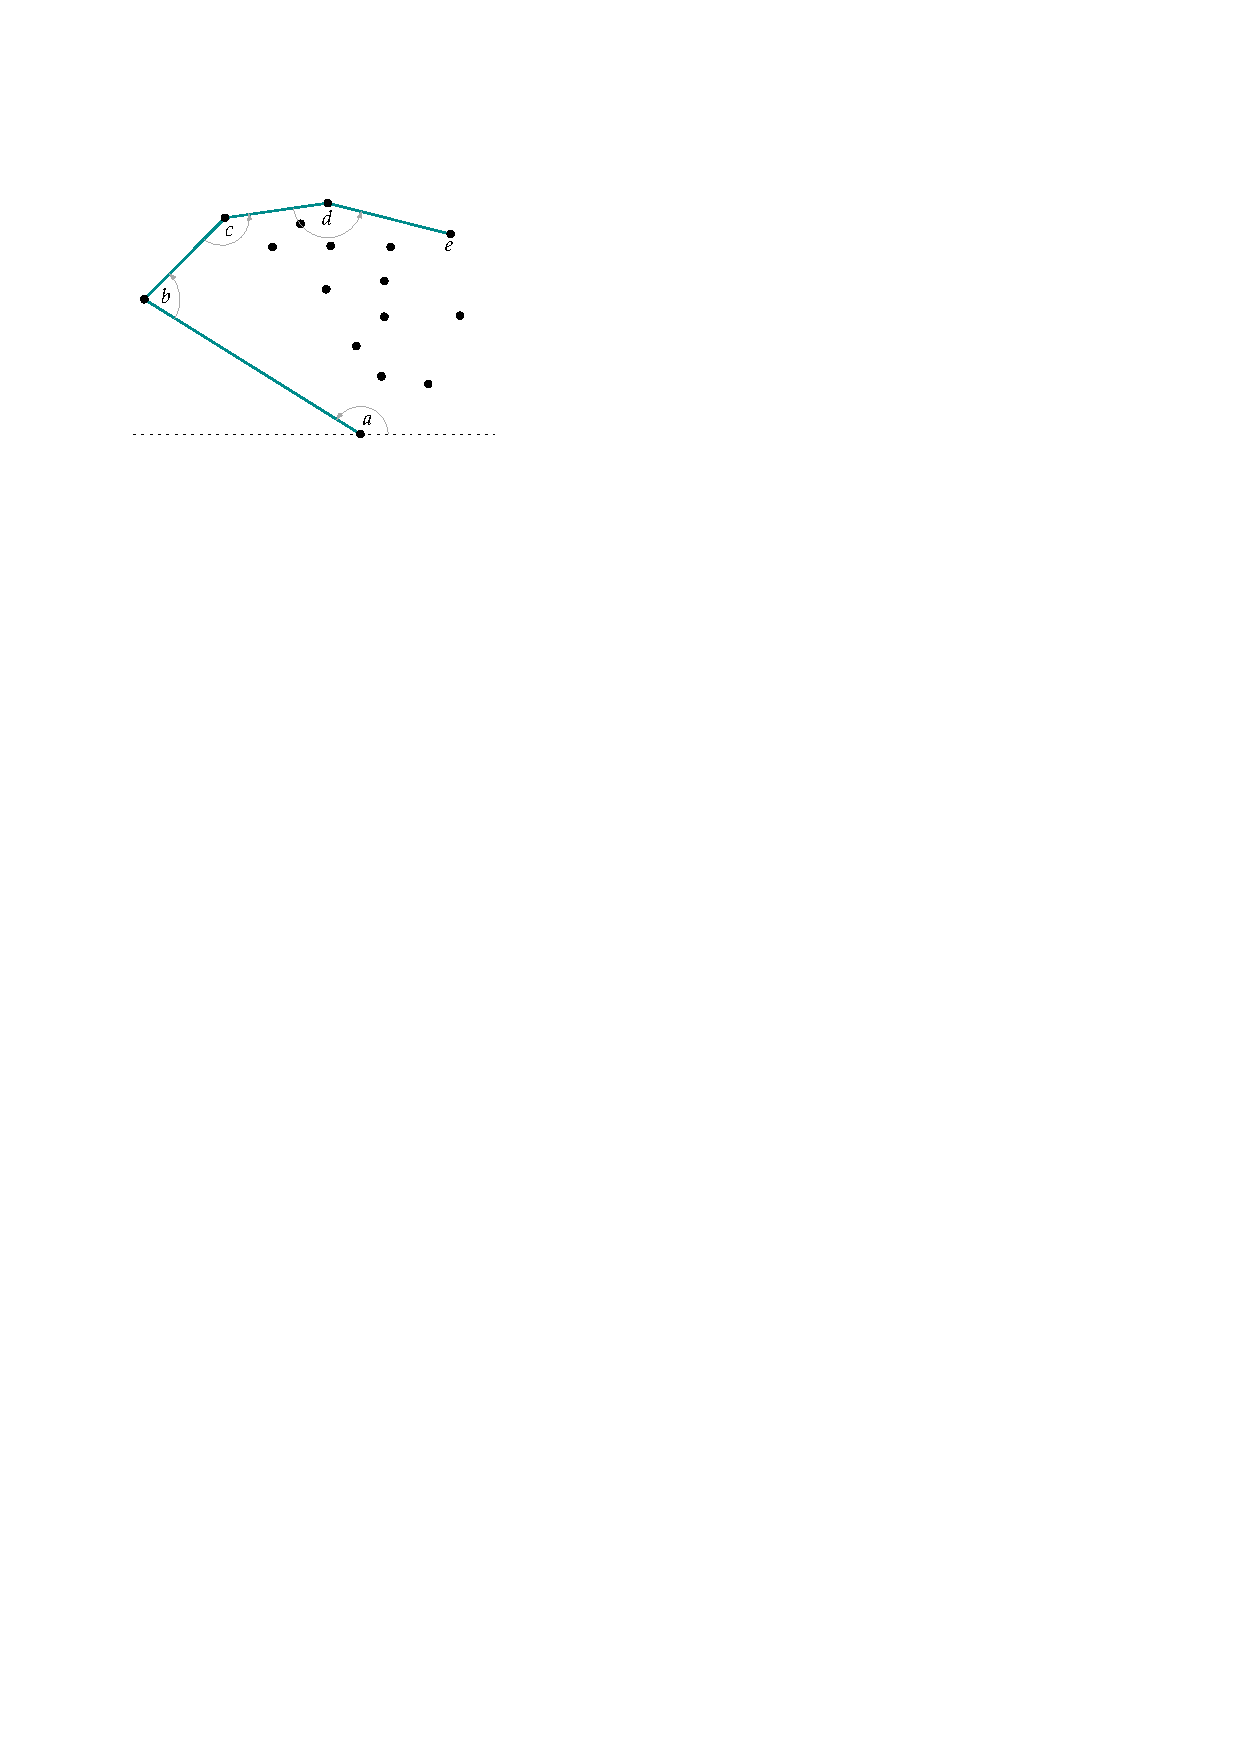
\includegraphics[width=0.6\linewidth]{figs/giftwrapping}
  \caption{First four steps of the gift wrapping algorithm to compute the convex hull.}
\label{fig:giftwrapping}
\end{figure}
It begins with a point that is guaranteed to be on conv($S$) (we can take an `extreme', such as $a$ in Figure~\ref{fig:giftwrapping} that is the point with the lowest $y$-coordinate), and then picks the point in $S$ for which the polar angle between the horizontal line and that point (at $a$) is the smallest.
Then for $b$, the polar angle is calculated from the line $ab$.
The algorithm terminates when $a$ is visited again.

%
Properties:
\\
\begin{tabular}{@{}ll@{}}
\toprule
P1. & The solve polygon is guaranteed to be regular.  \\  
P2. & A subset of $S$, or all of them, forms the region. \\ 
P3. & Outlier part of the region. \\ 
P4. & One component.  \\ 
P5. & No holes in the region.  \\  
\bottomrule
\end{tabular}



%%%%%%%%%%%%%%%%%%%%
%
\section{Moving arm}




%%%%%%%%%%%%%%%%%%%%
%
\section{$\chi$-shape}

%%%%%%%%%%%%%%%%%%%%
%
\section{$\alpha$-shape}

%%%%%%%%%%%%%%%%%%%%
%
\section{Notes \& comments}

The properties listed in Section~\ref{sec:properties} are taken, and slightly adapted, from \citet{Galton06}. 

The gift wrapping algorithm to compute the convex hull of a set of points in $\mathbb{R}^2$ is from \citet{Jarvis73}.

%%%%%%%%%%%%%%%%%%%%
%
\section{Exercises}

\begin{enumerate}
  \item When converting isolines to a TIN, what main ``problem'' should you be aware of? Describe \emph{in details} one algorithm to convert isolines (given for instance in a \emph{shapefile}) to a TIN and avoid this problem.
  \item How would the isocontours of a 2.75D terrain look like?
  \item In Section~\ref{sec:structuring}, it is mentioned that merging the segments will form on polygon. But how to ensure that the orientation of that resulting curve is consistent, that it is for instance having higher terrains on the right?
  \item Given a raster terrain (GeoTiff format) that contains several cells with \texttt{no\_data} values, describe the methodology you would use to extract contour lines from it. As a reminder, contours lines should be closed curves, except at the boundary of the dataset.
\end{enumerate}